\documentclass[12pt]{article}
\usepackage{amsmath,amsthm,amssymb,enumitem,tikz}
\usepackage[margin=.75in]{geometry}
\pagestyle{empty}

\usetikzlibrary {shapes.geometric}

\newcommand{\C}{\mathbb{C}}
\newcommand{\R}{\mathbb{R}}
\newcommand{\Z}{\mathbb{Z}}
\newcommand{\abar}{\overline{a}}
\newcommand{\aut}{\operatorname{aut}}

\setlength{\parindent}{0pt}
\begin{document}
	\begin{center}
		{\Large \bf Math 425 Objective Group-9 Exercises}
	\end{center}
	\section*{Purpose}
	\begin{itemize}
		\item This document is intended to provide additional opportunities to complete the objective
		
		\textbf{Group-9:}  Compute the group and Cayley table for the symmetry group of a given shape, and determine which of our standard groups it is isomorphic to.
	\end{itemize}
	\section*{Task}
	\begin{itemize}
		\item If you have not yet earned a \textbf{Satisfactory} or \textbf{Exceptional} mark on an exercise labeled with the objective here, you may submit a single one of the following exercises, that you have not yet attempted via Canvas by 4pm on any following Wednesday.
		\item I strongly recommend you use LaTeX to typeset your proofs.
		\item You may work in groups but everyone should submit their own assignment written in their own words.  Do NOT copy your classmates.
		\item Allowed resources: our textbook, classmates, your notes, videos linked in Canvas.
		\item Unacceptable resources: anything you find on an internet search. Do NOT use a homework help website (e.g., Chegg). Their solutions are often wrong or use incorrect context.  I want you to practice making arguments that are yours. Take some ownership.
	\end{itemize}
	\section*{Criteria}
	All items will earn a score using the following scale:
	\begin{itemize}
		\item \textbf{Exceptional} - Solution is succinct, references the correct theorems and definitions, and is entirely correct.
		\item \textbf{Satisfactory} - Solution is nearly correct. It still references the correct theorems and definitions. 
		It may be longer than necessary, have minor errors, or have some grammatical mistakes.
		\item \textbf{Unsatisfactory} - Solution has major errors, references content not covered in class or in the textbook, or is incomplete in some major way.
	\end{itemize}
	Recall from the syllabus
	\begin{itemize}
		\item If you earn either an \textbf{Exceptional} or \textbf{Satisfactory} mark on an objective exercise (labeled Intro-, Group-, or Ring-) then you may consider that item complete. 
		\item If you earn an \textbf{Unsatisfactory} mark on an objective exercise (labeled Intro-, Group-, or Ring-) then you have not yet completed this objective.
		\item You may submit a new attempt at completing that objective on a future Wednesday. You must select a new exercise listed under the given objective, you cannot resubmit a version you have attempted previously.  The only limit you have on number of attempts is the number of exercises available for the objective.
	\end{itemize}
	
	
	\newpage
	Name: \underline{\hspace*{3in}}
	\vskip .25in
	
	\textbf{(Group-9.2)} Consider the diamond as follows. (For clarity: all edges and the horizontal diagonal of length 1.)

	\begin{center}
		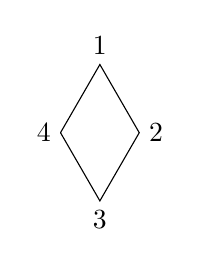
\begin{tikzpicture}
			\setlength{\unitlength}{1in}
			\draw (0,0) -- (.5,.866) -- (1,0) -- (.5,-.866) -- (0,0) node[anchor=east] {4} (.5,.866) node[anchor=south] {1} (1,0) node[anchor=west]{2} (.5,-.866) node[anchor=north] {3};
		\end{tikzpicture}
	\end{center}
	
	\begin{enumerate}[label=(\alph*)]
		\item Using $r$ as rotation by $90^\circ$ and $f$ as a flip along the vertical axis at the center of this figure, as in $D_4$, write all of the symmetries of this diamond in terms of $r$ and $f$.  That is, which combinations of $r$ and $f$ return this shape to the same location, possibly with the numbers swapping?
		\vskip 2in
		\item Write and complete a Cayley table for the group you found in part (a).
		\vfill 
		\item What group ($\Z_n$, $\Z_m\times\Z_n$, $S_n$, $D_n$, $\dots$) is this group of symmetries isomorphic to? Specifically you should be considering the following questions: What is the order of the group? Is this group cyclic? If it is not cyclic is it at least abelian?
		\vskip 1in
	\end{enumerate}
	
	\newpage
	Name: \underline{\hspace*{3in}}
	\vskip .25in
	
	\textbf{(Group-9.3)} Consider the square as follows. (For clarity: the double-marked edges of the square shown are painted blue. And for the shape to remain the same, the blue edges must remain blue.)

	\begin{center}
			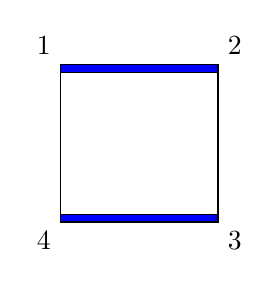
\begin{tikzpicture}
				\draw (0,0) rectangle (2,2) node[anchor=south west] {2} (2,0) node[anchor=north west] {3} (0,0) node[anchor=north east] {4} (0,2) node[anchor=south east] {1};
				\draw[fill=blue] (0,.1) rectangle (2,0);
				\draw[fill=blue] (0,1.9) rectangle (2,2);
			\end{tikzpicture}
	\end{center}
	
	\begin{enumerate}[label=(\alph*)]
		\item Using $r$ as rotation by $90^\circ$ and $f$ as a flip along the vertical axis at the center of this figure, as in $D_4$, write all of the symmetries of this square in terms of $r$ and $f$.  That is, which combinations of $r$ and $f$ return this shape to the same location, possibly with the numbers swapping?
		\vskip 2in
		\item Write and complete a Cayley table for the group you found in part (a).
		\vfill 
		\item What group ($\Z_n$, $\Z_m\times\Z_n$, $S_n$, $D_n$, $\dots$) is this group of symmetries isomorphic to? Specifically you should be considering the following questions: What is the order of the group? Is this group cyclic? If it is not cyclic is it at least abelian?
		\vskip 1in
	\end{enumerate}
	
	\newpage
	Name: \underline{\hspace*{3in}}
	\vskip .25in
	
	\textbf{(Group-9.4)} Consider the dart as follows. (For clarity: this is an isocoles triangle with a bend in the middle of the bottom.)

	\begin{center}
		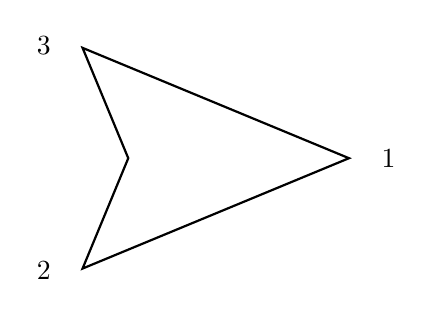
\begin{tikzpicture}
			\setlength{\unitlength}{1in}
			   \node[dart, draw, black, thick, inner sep=.25in]			(d) {};
			   \node [right=.1in] at (d.tip) {1};
			   \node [left=.1in] at (d.right tail) {2};
			   \node [left=.1in] at (d.left tail) {3};
		\end{tikzpicture}
	\end{center}
	
	\begin{enumerate}[label=(\alph*)]
		\item Tell me what you mean by $r$ and $f$ when finding the symmetry group of this shape, and tell me what the symmetry group is.
		\vskip 2in
		\item Write and complete a Cayley table for the group you found in part (a).
		\vfill 
		\item What group ($\Z_n$, $\Z_m\times\Z_n$, $S_n$, $D_n$, $\dots$) is this group of symmetries isomorphic to? Specifically you should be considering the following questions: What is the order of the group? Is this group cyclic? If it is not cyclic is it at least abelian?
		\vskip 1in
	\end{enumerate}
\end{document}